%' Directed acyclic graph (DAG) with arrow text annotations
%'
%' @src: Figure 6 in Theory-Driven Analysis of Intra-individual Dynamics 
%' @url: https://yongfu.name/intra/main.pdf

\documentclass[12pt,preview,border=0]{standalone}
\usepackage[paperheight=10cm,paperwidth=10cm]{geometry}
\usepackage{graphicx}
\usepackage{amsmath}
\usepackage{kmath,kerkis}
\usepackage{tikz}
\usetikzlibrary{arrows,automata,positioning}

\begin{document} 
\begin{center}
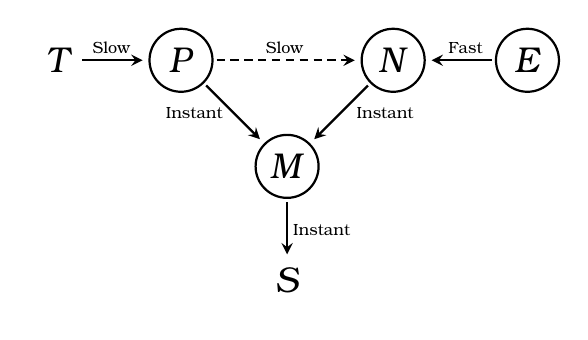
\begin{tikzpicture}[
	> = stealth, % arrow head style
	shorten > = 1pt, % don't touch arrow head to node
	auto,
	node distance = 2cm, % distance between nodes
	thick, % line style
	U/.style={circle, draw=black, inner sep=1.8pt, outer sep=1.5pt, minimum size=8mm, font=\Large},  %draw=black, fill=white
	O/.style={circle, inner sep=3.4pt, outer sep=-3pt, minimum size=8mm, font=\Large},              %draw=white, fill=white
	]
	
	% Nodes and their relative positions
	\node[U] (M) {$M$};
	\node[O] (S) [below = .7 of M] {$S$};
	\node[U] (P) [above left  = 1 of M] {$P$};
	\node[U] (N) [above right = 1 of M] {$N$};
	\node[U] (E) [right = .8 of N] {$E$};
    \node[O] (T) [left  = .8 of P] {$T$};

	% Paths connecting nodes
    \path[->] (T) edge node[above,scale=.65]{Slow ~}    (P);
	\path[->] (E) edge node[above,scale=.65]{~ Fast}    (N);
    \path[->] (P) edge node[left, scale=.65]{Instant ~} (M);
	\path[->] (N) edge node[right,scale=.65]{~ Instant} (M);
	\path[->] (M) edge node[right,scale=.65]{Instant}   (S);

    \path[->] (P) edge[densely dashed] node[above,scale=.65]{Slow ~} (N);
	
\end{tikzpicture}
	

\end{center}\end{document}
